\documentclass[a4paper,13pt]{book}
\usepackage[centertags]{amsmath}
\usepackage{amscd}
\usepackage{amsthm}
\usepackage{amssymb}
%\usepackage{array}
\usepackage{enumerate}
%\usepackage{xypic}
%\usepackage[dvips]{graphics}
%\usepackage{moreverb}
\usepackage{multicol}
\usepackage{hyperref}
\usepackage[english]{babel}
%\usepackage{epsfig}
%\usepackage{rotating}
%\usepackage[all]{xy}
\usepackage{color}
\usepackage{tikz}
\usepackage{tabls} %per tenir m{\'e}s control sobre l'espai en les taules nom{\'e}s cal aquest paquet
\usepackage{indentfirst} %per comen\c{c}ar primer parragraf de seccio o capitol amb indent
\usepackage{imakeidx}
\makeindex

\usepackage[T1]{fontenc}
% \usepackage[sc]{mathpazo}
\linespread{1.1} % Palatino needs more leading (space between lines)

\usepackage[latin1]{inputenc}
\usepackage[twoside,bindingoffset=1cm]{geometry}


%%%%%%%%%%%%%%%%%%%%%%%%%%%%%%%%%%%%%%%%%%%%%%%%%%%%%%%%%%%%%%%%%%%%%%%%%
% theorem environments
%%%%%%%%%%%%%%%%%%%%%%%%%%%%%%%%%%%%%%%%%%%%%%%%%%%%%%%%%%%%%%%%%%%%%%%%%

\newtheorem{defn0}{Definition}[chapter]
\newtheorem{prop0}[defn0]{Proposition}
\newtheorem{thm0}[defn0]{Theorem}
\newtheorem{lemma0}[defn0]{Lemma}
\newtheorem{corollary0}[defn0]{Corollary}
\newtheorem{example0}[defn0]{Example}
\newtheorem{remark0}[defn0]{Remark}
\newtheorem{conjecture0}[defn0]{Conjecture}

\newenvironment{definition}{ \begin{defn0}}{\end{defn0}}
\newenvironment{proposition}{\bigskip \begin{prop0}}{\end{prop0}}
\newenvironment{theorem}{\bigskip \begin{thm0}}{\end{thm0}}
\newenvironment{lemma}{\bigskip \begin{lemma0}}{\end{lemma0}}
\newenvironment{corollary}{\bigskip \begin{corollary0}}{\end{corollary0}}
\newenvironment{example}{ \begin{example0}\rm}{\end{example0}}
\newenvironment{remark}{ \begin{remark0}\rm}{\end{remark0}}
\newenvironment{conjecture}{\begin{conjecture0}}{\end{conjecture0}}

\newcommand{\defref}[1]{Definition~\ref{#1}}
\newcommand{\propref}[1]{Proposition~\ref{#1}}
\newcommand{\thmref}[1]{Theorem~\ref{#1}}
\newcommand{\lemref}[1]{Lemma~\ref{#1}}
\newcommand{\corref}[1]{Corollary~\ref{#1}}
\newcommand{\exref}[1]{Example~\ref{#1}}
\newcommand{\secref}[1]{Section~\ref{#1}}
\newcommand{\remref}[1]{Remark~\ref{#1}}
\newcommand{\conjref}[1]{Conjecture~\ref{#1}}


\newcommand{\OO}{\texorpdfstring{\,\vcenter{\hbox{
\includegraphics[scale=0.2]{pieces/pieces_O.pdf}}}\,}O}
\newcommand{\TT}{\texorpdfstring{\,\vcenter{\hbox{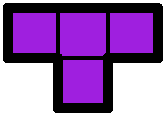
\includegraphics[scale=0.2]{pieces/pieces_T.pdf}}}\,}T}
\newcommand{\LL}{\texorpdfstring{\,\vcenter{\hbox{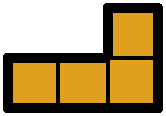
\includegraphics[scale=0.2]{pieces/pieces_L.pdf}}}\,}L}
\newcommand{\JJ}{\texorpdfstring{\,\vcenter{\hbox{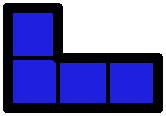
\includegraphics[scale=0.2]{pieces/pieces_J.pdf}}}\,}J}
\renewcommand{\SS}{\texorpdfstring{\,\vcenter{\hbox{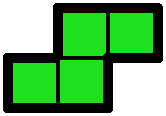
\includegraphics[scale=0.2]{pieces/pieces_S.pdf}}}\,}S}
\newcommand{\ZZ}{\texorpdfstring{\,\vcenter{\hbox{
\includegraphics[scale=0.2]{pieces/pieces_Z.pdf}}}\,}Z}
\newcommand{\II}{\texorpdfstring{\,\vcenter{\hbox{
\includegraphics[scale=0.2]{pieces/pieces_I.pdf}}}\,}I}
\newcommand{\ALL}{\II, \allowbreak \OO, \allowbreak \TT, \allowbreak \SS, \allowbreak \ZZ, \allowbreak \JJ, \allowbreak \LL}

\NewDocumentCommand{\cell}{O{i} O{j}}{
 \langle #1, #2 \rangle
}
\NewDocumentCommand{\piece}{O{t} O{\theta} O{i} O{j} O{f}}{
 (#1, \allowbreak #2, \allowbreak \langle #3, \allowbreak #4 \rangle,  \allowbreak #5 )
}


\newcommand{\texttheo}[1]{\textnormal{\textsf{#1}}}
\newcommand{\tetris}[1]{\textsc{Tetris}[#1]\xspace}
\newcommand{\npc}{\textnormal{\textsf{NP-complete} }}
\newcommand{\pp}{\textnormal{\textsf{P}}}
\newcommand{\nph}{\textnormal{\textsf{NP-hard} }}
\newcommand{\survival}{\texttheo{survival }}
\newcommand{\clearing}{\texttheo{clearing }}
%%%%%%%%%%%%%%%%%%%%%%%%%%%%%%%%%%%%%%%%%%%%%%%%%%%%%%%
% environments per la intro i pel resum en catal{\`a} %
%%%%%%%%%%%%%%%%%%%%%%%%%%%%%%%%%%%%%%%%%%%%%%%%%%%%%%%

%intro


\newtheorem{th1}{Theorem}
\newtheorem{prop1}[th1]{Proposition}
\newtheorem{cor1}[th1]{Corollary}
\newtheorem{lem1}[th1]{Lemma}
\newtheorem{de1}[th1]{Definition}
%catala

\newtheorem{th2}{Teorema}
\newtheorem{prop2}[th2]{Proposici{\'o}}
\newtheorem{cor2}[th2]{Corol{\cdot}lari}
\newtheorem{lem2}[th2]{Lema}

%%%%%%%%%%%%%%%%%%%%%%%%%%%%%%%%%%%%%%%%%%%%%%%%%%%%%%%%%%%%%%%%%%%%%%%%%%%
%%%% local definitions for this paper
%%%%%%%%%%%%%%%%%%%%%%%%%%%%%%%%%%%%%%%%%%%%%%%%%%%%%%%%%%%%%%%%%%%%%%%%%%%






%%%%%%%%%%%%%%%%%%%%%% aix{\`o} pels headings %%%%%%%%%%%%%%%%%%%%%%%%
\usepackage{fancyhdr}
\pagestyle{fancy}
\renewcommand{\chaptermark}[1]{\markboth{#1}{}}
\renewcommand{\sectionmark}[1]{\markright{\thesection\ #1}}
\fancyhf{} \fancyhead[LE,RO]{\bfseries\thepage}
\fancyhead[LO]{\bfseries\rightmark} \fancyhead[RE]{\bfseries\leftmark}

\def\paginaenblanc{\newpage%
\thispagestyle{empty}%
\vspace*{2cm}%
\newpage%
\thispagestyle{empty}%
}


%%%%%%%%%%%%%%%%%%%%%%%%%%%%%%%%%%%%%%%%%%%%%%%%%%%%%%%%%%%%%%%%%%%%%%%%%
% aux commands
%%%%%%%%%%%%%%%%%%%%%%%%%%%%%%%%%%%%%%%%%%%%%%%%%%%%%%%%%%%%%%%%%%%%%%%%%
%==========================================================================
% macros to support private authors' notes
%==========================================================================
\newif\ifprivate
\privatetrue
\def\xbar{\vskip0.09in\hrule\vskip0.06in}
\def\private#1{\ifprivate \xbar {\em #1} \xbar
\else \fi}
\def\huh{\ifprivate ??? \marginpar{\Huge ???}
\else \fi}
\def\???{\ifprivate {\bf {???}} \marginpar{\begin{center}{\Huge {\bf ?}}\end{center}}
\else \fi}
%\def\???{\ifprivate {\bf {???}} \marginpar{{\Huge {\bf ?}}}
%\else \fi}
\marginparsep1mm
\def\nota#1{\ifprivate  $\clubsuit$ \marginpar{\parbox[t]{2.4cm}{\begin{center}\tiny #1\end{center}}}
\else \fi}
\def\comment#1{\ifprivate \marginpar{\parbox[t]{2.4cm}{\begin{center}\tiny #1\end{center}}}
\else \fi}
%\def\nota#1{\ifprivate  $\clubsuit$ \marginpar{\parbox[t]{1.8cm}{\tiny #1}}
%\else \fi}
\def\privateeject{\ifprivate\eject\fi}
%\def\???{{\bf {???}} \marginpar{{\Huge {\bf ?}}} }
%%%%%%%%%%%%%%%%%%%%%%%%%%%%%%%%%%%%%%%%%%%%%%%%%%%%%%%%%%%%%%%%%%%%%%%%%%

%%%%%%%%%%%%%% definicions cap{\'\i}tol ""%%%%%%%%
%%%%%%%%%%%%%%%%%%%%%%%%%%%%%%%%%%
\def\av{\underline{a}}

\def\Zr{\mathbb Z^r} \def\Nr{\mathbb N^r}
\def\xv{\underline{x}}
\def\yv{\underline{y}}
\def\zv{\underline{z}}

\newcommand{\Proj}{\operatorname{Proj}}
\newcommand{\Spec}{\operatorname{Spec}}


\def\HiRIM#1{H^i_{\mathcal M}(#1)}

\newcommand{\im}{\operatorname{Im}}
\renewcommand{\ker}{\operatorname{Ker}}
\newcommand{\grade}{\operatorname{grade}}
\newcommand{\Ext}{\operatorname{Ext}}
\newcommand{\Hom}{\operatorname{Hom}}
\newcommand{\m}{\mathfrak m}
\newcommand{\n}{\mathfrak n}
\newcommand{\M}{\mathfrak m}
%\newcommand{\cL}{{\mathcal L}}
\newcommand{\cP}{{\mathcal P}}
\newcommand{\cE}{{\mathcal E}}
\newcommand{\cS}{{\mathcal S}}
\newcommand {\PP}{\mathbb{P}}

\def\p{\mathfrak{p}}
\def\q{\mathfrak{q}}
\DeclareMathOperator{\de}{deg}

\DeclareMathOperator{\Hl}{H}
 \DeclareMathOperator{\h}{h}


%%%%%%%%%%%%%%%%%%%%%%%%%%%%%%%%%%%%%%%%%%%%%%%%%%%%%%%%%%%%%%%%%%%%%%%%%
%%%%%%%%%%%%%%%%%%%%%%%%%%%%%%%%%%%%%%%%%%%%%%%%%%%%%%%%%%%%%%%%%%%%%%%%%
%%%%%%%%%%%%%%%%%%%%%%%%%%%%%%%%%%%%%%%%%%%%%%%%%%%%%%%%%%%%%%%%%%%%%%%%%
%%%%%%%%%%%%%%%%%%%%%%%%%%%%%%%%%%%%%%%%%%%%%%%%%%%%%%%%%%%%%%%%%%%%%%%%%
%%%%%%%%%%%%%%%%%%%%%%%%%%%%%%%%%%%%%%%%%%%%%%%%%%%%%%%%%%%%%%%%%%%%%%%%%
%%%%%%%%%%%%%%%%%%%%%%%%%%%%%%%%%%%%%%%%%%%%%%%%%%%%%%%%%%%%%%%%%%%%%%%%%
%%%%%%%%%%%%%%%%%%%%%%%%%%%%%%%%%%%%%%%%%%%%%%%%%%%%%%%%%%%%%%%%%%%%%%%%%
%%%%%%%%%%%%%%%%%%%%%%%%%%%%%%%%%%%%%%%%%%%%%%%%%%%%%%%%%%%%%%%%%%%%%%%%
%%%%%%%%%%%%%%%%%%%%%%%%%%%%%%%%%%%%%%%%%%%%%%%%%%%%%%%%%%%%%%%%%%%%%%%%
\begin{document}

\makeatletter
\def\old@comma{,}
\catcode`\,=13
\def,{%
  \ifmmode%
    \old@comma\discretionary{}{}{}%
  \else%
    \old@comma%
  \fi%
}
\makeatother

\section{Game Definitions}

In \cite{TIH} we can find a formalization of the Tetris game and a decisional/functional problem associated to it. Since the video game is played in finite board and a player can't win, the definition of the game introduces some variations to build a complexity problem.

In \cite{TT,TWFP,TCB,CTV,AVG} game variations are introduced without any formalization of the new emerging problems. We are going to provide a generalized Tetris game definition, following \cite{TIH}, which aims to include all possible game variations and the combination of these. Right after defining each part of the game, an example will be given of what be in the video game and what it is in the definition of \cite{TIH}. We will refer to \emph{video game} and \emph{base tetris} respectively.

A \emph{Tetris game} will refer to the hole game with its rules, configurations, pieces, ... and a \emph{tetris match} will refer to a concrete Tetris game instance (the sequence of moves that a player would play). 

\begin{definition} \index{board}
  A \emph{board} \emph{B} is an $n$ by $m$ grid. Each cell $\cell$, $i = 1\dots n$, $j = 1\dots m$ is \emph{filled} or \emph{unfilled}.
\end{definition}

The board will be indexed from bottom to top and from left to right. The cell $\cell[1][1]$ is in the bottom left of the board and $\cell[n][m]$ is the top right-most cell.

In some results, the authors impose that the initial configuration must be constructible with the pieces and the rules of the game. This is that the initial configuration can be reached, with the game rules, from an empty board and an appropriate pieces sequences. Others, the only condition that is imposed on the initial configuration is that it can't have filled rows. We will not impose the board to be constructible, (parlem despres).

\begin{example} 
  \begin{itemize}
    \item \textbf{Video game:} the board size is typcaly a unfilled 10x20 board.
    \item \textbf{Base Tetris: } the board size has arbitrary dimensions.
  \end{itemize}
\end{example}


Tetris classical pieces are made up by attaching 4 squares. In the variations we can find pieces types, in a game there are usually pieces with the same number of cubes. A general Tetris piece made up with $k$ cells is:

\begin{definition} \index{$k$-omino} \index{polymonio}
  A \emph{$k$-omino} is a piece made up of $k$ unit squares joined edge to edge. A \emph{polyomino} is a $k$-omino for some $k$.
\end{definition}

For $k= 1,2,3,4,5$ the $k$-omio pieces are called respectively: \emph{monomino}, \emph{domino}, \emph{tromino}, \emph{tetromino} and \emph{pentomino}.

\begin{definition} \index{piece!types}
  The \emph{piece types} $T$ is a set of polyominos. If $T$ contains all the $k$-omions we will write $T_k$.
\end{definition}

\begin{example} The \textbf{video game} and the \textbf{base Tetris} have the same  pieces types $T_4 = \{ \ALL \}$, all the tetrominoes.
\end{example}

Given the pieces and the board, we can now define how a piece interacts with a board. 

\begin{definition} \index{piece!state} \index{piece}
 A \emph{piece state} in a board $B$ is a tuple $ P = \piece$ where:
  \begin{itemize}
    \item $t \in T$, a polyomino.
    \item $\theta$ the \emph{orientation}, the number of degrees clockwise from the original piece. $ \theta \in \lbrace 0^\circ, 90^\circ, 180^\circ, 270^\circ \rbrace $.
    \item $\cell$ is the \emph{position} of the piece in of $B$
    \item  $f$ indicates if the piece is \emph{fixed} or \emph{unfixed} in B.
  \end{itemize}

  We will refer to a piece sate as \emph{piece}.
   
\end{definition}


\begin{definition}
  Given a piece type $t$ and a board $B$, the piece $P_0 = \piece[t][0^\circ][n][\lfloor m / 2 \rfloor][\text{unfixed}]$ is the \emph{initial state} of the piece type of $t$ in the board $B$.
\end{definition}

The idea is to have only one active piece in a Tetris match. Only the piece that is moving has a state because when a piece reaches the \emph{fixed} state the piece is automatically merged with the board, and then the next piece starts in its initial state. In order to define how a piece moves thought the board, we need to define some \emph{moves} for changing the piece state.

\begin{definition}
  A \emph{move} is a computable function $m(B, P) = P'$ that given a board $B$ and a piece $P$ outputs a new piece $P'$. The following moves can be applied to an unfixed piece $P = \piece[t][\theta][i][j][\text{unfixed}]$. 
  \begin{itemize}
    \item $r_+$ a \emph{clockwise rotation:} if the rotated piece does not overlap with an occupied cell of the board, the output is 
      $$r_+ (B, \piece[t][\theta][i][j][\text{unfixed}]) = \piece[t][\theta + 90^\circ][i][j][\text{unfixed}]$$

    \item $r_-$ a \emph{counterclockwise rotation:} the same but counterclockwise rotation. 

    \item $s_l$ a \emph{slide to the left:} if all the board cells adjacent to de left of the piece are not occupied, the output is:
      $$s_l (B, \piece[t][\theta][i][j][\text{unfixed}]) = \piece[t][\theta][i][j-1][\text{unfixed}]$$
    \item $s_r$ a \emph{slide to the right:} analogous to the slide to the left.

    \item $d$ a \emph{drop by one row:} if all the board cells bellow the piece are not occupied the output is:
      $$d (B, \piece[t][\theta][i][j][\text{unfixed}]) = \piece[t][\theta][i-1][j][\text{unfixed}]$$

    \item $f$ a \emph{fix:} if any of the board cells bellow the piece is occupied, the output is:
      $$f (B, \piece[t][\theta][i][j][\text{unfixed}]) = \piece[t][\theta][i][j][\text{fixed}]$$
  \end{itemize}
  If the pre-conditions of a move are satisfied, the move is said to be \emph{legal}. If any of the conditions are not satisfied the move is \emph{illegal}.
\end{definition}

All the conditions can be computed in $\mathcal{O}(1)$, because only a constant numbers of cells are need to be visited every time. Let's now define the \emph{trajectory} of a piece type in a Tetris game. Intuitively the trajectory starts when the piece is given to the player, consists on a sequence of legal moves and ends when he fixes the piece in the board. 


\begin{definition}
 Let $B$ be a board and $t$ a piece type. Let $P_0$ be the initial state of the piece type $t$. Then a sequence of $k$ moves $\sigma = (m_1, ..., m_k)$ to the piece state after $i$ moves is a \emph{trajectory} if:

 \begin{itemize}
  \item the move $m_i$ over $P_i$ is a legal move for all $i = 1 \dots k$
  \item and $m_k = f$ is a \emph{fix} move.
 \end{itemize}
 
 Where $P_{i+1} = m_i(P_i)$ is the piece stat in $B$ after $i$ moves.
\end{definition}

The number of moves of a trajectory could be limited by $\mathcal{O}(n \cdot m)$?

With a board and a trajectory we need to define how we merge both. The resulting board will be the merged board. 

\begin{definition}
  Given a board $B$ and trajectory $\sigma = (m_1, ..., m_k)$ of a given piece type $t$ the \emph{merged game board} $B'$ is defined as follows:
  \begin{enumerate}
    \item $B'$ is initially $B$.
    \item The cells of $B$ corresponding to the last piece state of the trajectory are filled in $B'$.
    \item For every filled row $r$ of $B'$:
      \begin{enumerate}
        \item Replace each row $r' > r$ by $r'+1$.
        \item Clear (set all cells to unfilled) of row $m$.
      \end{enumerate}
  \end{enumerate}
\end{definition}

We have now all the components of a Tetris match.

\begin{definition}
  Given a board $B$ and a sequence of $k$ pieces types $P = (t_1,\dots,t_k)$ a \emph{Tetris match} $\Sigma$ is a sequence
  $$ B = B_0, \sigma_1, B_1, \sigma_2, B_2, \dots  \sigma_q, B_q, \; \; q \leq k$$ 
  where:
  \begin{itemize}
    \item $\sigma_i$ is a trajectory of the piece type $t_i$ in the board $B_{i-1}$.
    \item $B_{i+1}$ is the merged board from $B_i$ and $\sigma_i$.
    \item $q < k$ iff doesn't exist any trajectory $\sigma_{q+1}$ from de board $B_q$ with the piece type $t_{q+1}$. In this case we say the game is a \emph{loss}.
  \end{itemize}
\end{definition}

\section{Problem}

All the problems share the same formulation of the problem. The \textsc{Tetirs} problem is:

\begin{itemize}
  \item \textbf{Input} (\textit{a Tetris game}) : $\mathcal{G} = (B,(t_1,\dots,t_k))$ an initial board and a sequence of $k$ pieces types.
  
  \item \textbf{Output} : Does exist a match $\Sigma$ such that $\Phi ( \mathcal{G}, \Sigma )$ holds? 
\end{itemize}

Where $\Phi(\mathcal{G},\Sigma)$ is computable objective function that only takes into account the final state of the pieces, ignoring the piece trajectory (\emph{checkable and acyclic}). 


We will divide the problem variants classification in two parts: variations on the objective function and variations on the game formulation.

\subsection{Objective functions} 

Will refer to the \textsc{Tetris} problem with the objective function $\Phi$ as $\textsc{Tetris} [ \Phi ]$. The following are objective functions:

\begin{itemize}
  \item \texttheo{k-cleared-rows}: in the game $\mathcal{G}$, does $\sigma$ clear at least $k$ rows?
  \item \texttheo{k-tetrises}: in the game $\mathcal{G}$, does $\sigma$ contain at least $k$ tetrises?
  \item \texttheo{h-height-filled}: in the game $\mathcal{G}$, does $\sigma$ never fill a cell above height $h$?
  \item \texttheo{p-placed-pices}: in the game $\mathcal{G}$, does $\sigma$ place at least $p$ pieces before losing.
\end{itemize} 

The two most popular variations are:

\begin{itemize} 
  \item \clearing: in the game $\mathcal{G}$, does $\sigma$ leave every cell of the board unfilled?
  \item \survival: is equivalent to \texttheo{n-height-filled}, where $n$ is the height of board $B$. This is finding a sequence $\Sigma$ that is not a loss.
\end{itemize}

\section{Game variations and Results}

Game variations are obtained tweaking definitions of the game. The following parameters of the game can be changed: 

\begin{itemize}
  \item \textbf{Pieces:} changing the pieces set of a Tetris game
  \item \textbf{Moves:} extending, reducing or changing the moves that can be applied to the pieces. 
  \item \textbf{Board:} fixing the board dimensions or impose restriction of the initial board.
  \item \textbf{Pieces sequences:} imposing restriction over the sequence of pieces.
\end{itemize}

The following papers provide results on Tetris and its variations.

\subsection{Tetris is hard, even to approximate}

The first results about Tetris complexity appear in \cite{TIH}. The results are the following:

\begin{theorem}
  Tetris is \nph to optimize (or approximate) with the objectives, \texttheo{k-cleared-rows}, \texttheo{k-tetrises} \texttheo{h-height-filled} and \texttheo{p-placed-pices}. It remains \nph even if:
  \begin{itemize}
    \item The player is restricted to two rotation/translation moves before each piece drops in height.
    \item Pieces are restricted to $\{\LL, \SS, \II, \OO\}$ or $\{\LL, \ZZ, \II, \OO\}$ plus at least one other piece.
    \item Losses are not triggered until after filled rows are cleared.
    \item Rotations follow any reasonable rotation model.
  \end{itemize}
\end{theorem}

A \emph{reasonable rotation model} is a generalization of the $\{r_+,r_-\}$ moves, extending the available rotations for a piece in a board. The two rotation functions are reasonable if some common sense conditions, defined in \cite{TIH}.

OPEN PROBLEMS?

\subsection{Total Tetris: Tetris with Monominoes, Dominoes, Trominoes, Pentominoes, ...}

In \cite{TT} a piece variation is introduced. $k$-\textsc{tris} changes the pieces types by changing the number of \emph{cells} ($k$) that form the piece types. The  set of pieces types in $k$-\textsc{tris} is all possible pieces of $k$ cells.

In the classical Tetris is $4$-\textsc{tris}, where 7 possible pieces can be built. For $k = 1$ one piece types is available (a cell), for $k=2$ also one piece type is only available (two adjacent cells), and so on. 

The formalization is almost the same as the one described in this document. The set of piece types varies depending on $k$, and each respective center. Varies depending on $k$. The \emph{moves} describing each piece state transformation is appropriately modified to fit the new piece types. Results are presented in Table~\ref{tab:tt} 


\subsubsection{Without rotation}

If we remove $r_+, r_-$ from the moves set we obtain Tetris without rotation, were the player cannot rotate pieces. Since the orientation in the \emph{initial position} of a piece is always $\theta = 0^\circ$, we can fix this by adding the initial orientation of each piece in the Tetris game instance.

\textbf{Input} (\textit{a Tetris game}): $\mathcal{G} = (B,(t_1,\theta_1, \dots,t_k,\theta_1))$ an initial board and a sequence of $k$ pieces types and its initial orientation.


The rest of the game is exactly the same. The results are presented in Table~\ref{tab:tt} 

\begin{table}[h!]
\centering
\label{tab:tt}
\begin{tabular}{|c || c | c || c | c ||} 
 \hline
  & \multicolumn{2}{| c ||}{\survival} & \multicolumn{2}{| c |}{\clearing} \\
 \hline
  & with rotation & no rotation & with rotation & no rotation \\
 \hline               
 $k = 1$ & \pp  & \pp  & \pp  & \pp \\ 
 \hline                             
 $k = 2$ & Open & Open & Open & \npc \\
 \hline                             
 $k = 3$ & Open & \npc & \npc & \npc\\
 \hline                             
 $k = 4$ & \npc & \npc & \npc & \npc\\
 \hline                             
 $k > 5$ & \npc & \npc & \npc & \npc\\
 \hline
\end{tabular}

\caption{\cite{TT} results with rotation}
\end{table}

OPEN PROBLEMS?

\subsection{Tetris is NP-hard even with O(1) rows or columns}

Following the variants introduced in \cite{TT}, in \cite{TCB} new variations are introduced. In  a $(\leq)k$-\textsc{tris} game, the set of pieces types is all possible pieces of $\leq k$ cells. Then we define the following problems:

\begin{itemize}
  \item $c$-\textsc{Column} $(\leq)k$-\textsc{tris}: $(\leq)k$-\textsc{tris} where the board width is fixed to $c$.
  \item $r$-\textsc{Row} $(\leq)k$-\textsc{tris}: $(\leq)k$-\textsc{tris} where the board height is fixed to $c$.
\end{itemize}

The rows and columns, respective, remain arbitrary. These two versions can be combined with the empty Tetris.

\begin{itemize}
  \item \textsc{Empty $(\leq)k$-\textsc{tris}}: $(\leq)k$-\textsc{tris} where all the board cells are initially unfilled.
\end{itemize}

Results with this variation are in Table~\ref{tab:tcb}

\begin{table}[h!]
\centering
\label{tab:tcb}
\begin{tabular}{|c | c | c | c | c |} 
 \hline
 Rows   & Columns & Empty  & Piece Sizes  & Complexity      \\
 \hline
 \hline
 $1   $ & $O(n) $ & no     & $O(n)    $ & strongly \nph   \\ \hline
 $1   $ & $O(n) $ & yes    & $O(n)    $ & linear          \\ \hline
 $1   $ & $O(n) $ & no     & $k       $ & linear          \\ \hline
 $2   $ & $O(n) $ & yes    & $O(n)    $ & strongly \nph   \\ \hline
 $3   $ & $O(n) $ & no     & $4       $ & Open            \\ \hline
 $4   $ & $O(n) $ & no     & $4       $ & strongly \nph   \\ \hline
 $O(n)$ & $1    $ & no     & $O(n)    $ & linear          \\ \hline
 $O(n)$ & $2    $ & no     & $O(n)    $ & polynomial      \\ \hline
 $O(n)$ & $3    $ & yes    & $O(n)    $ & strongly \nph   \\ \hline
 $O(n)$ & $3 - 7$ & no     & $4       $ & Open            \\ \hline
 $O(n)$ & $8+   $ & no     & $4       $ & strongly \nph   \\ \hline
 $O(n)$ & $8    $ & yes    & $\leq 65 $ & strongly \nph   \\
 \hline
\end{tabular}
\caption{\cite{TT} results table}
\end{table}

OPEN PROBLEMS?

\subsection{Tetris with Few Piece Types}

In \cite{TWFP} variations of the original problem with fewer pieces are introduced, we only use a subset of the 7 available pieces types of Tetris. 

\textbf{Main Result:} for every 2-sized subset of $\{\ALL\}$, Tetris \survival and \clearing is \nph under SRS.

SRS is a new reasonable rotation model, used in the demonstrations that allow more rotations. The possible piece states after a rotation are a superset of the rotation model used in the game definition.


Two new movement variants are introduced:

\begin{itemize}
  \item \texttheo{Hard-Drop}: when playing the Tetris video game, specially in the initial rounds of a game, the player can hard drop a piece in order to avoid dropping the piece one row at a time. \emph{drop} and \emph{fix} are removed from the set of moves, and \emph{hard-drop} is added. Hard-dropping a piece moves it maximally downward before fixing into place.
  \item \texttheo{20-G}:In this model, instead of periodically moving down one unit, all pieces move maximally down-ward instantly and on their own, and the player is not allowed to control how fast a piece moves downward. The player is still free to rotate or move the piece left or right before the piece locks. \emph{drop} move is removed, and the vertical position of the initial state of a piece is now the lowest possible.
\end{itemize}

\textbf{Result:} Tetris \texttheo{20-G} and Tetris \texttheo{Hard-Drop} is \npc  even if the pieces set is restricted to $\{ \II, \OO \}$ \cite{TWFP}. 


\textbf{Result:} if we allow the piece $\{ \TT \}$, the above result can be extended to \nph.



\section{Open Stuff}

A list of open variations, no one has explored.

\begin{itemize}
  \item \textbf{Hold-Function:} in this version the player has a \emph{box} to put aside a piece for a later use.
  \item \textbf{7-bag randomizer:} the pieces are presented to the player in sequences of 7 pieces. Each sequence must contain the 7 pieces (in the traditional version) in any order. 
  \item \textbf{Empty:} Tetris with the initial board unfilled.
\end{itemize}




\section{Related problems}

Other problems related to Tetris.

\subsection{Tetris and decidability}

In \cite{TAD}, they consider a variant of Tetris where the sequence of pieces (together with their orientation and horizontal position, which cannot be changed anymore) is generated by a finite state automaton. They show that it is undecidable, given such an automaton, and starting from an empty game board, whether one of the generated sequences leaves an empty game board.

Since we are dealing with pieces sequences of a regular language we cannot fix the board height, so in this version the board height is unbounded. The formal problem definition is:

\vspace{1em}
\textbf{Instance:} an empty board $B$ of width $w$ and $L$, a regular language describing sequences of Tetris pieces with their initial position and orientation. 

\textbf{Question:} is there a sequence in $L$ that leaves the game board empty after dropping all pieces into the empty board?
\vspace{1em}

This problem with a board of width of 10 is undecidable for sequences only of $\II$ (reduction from PCP), but with only $\OO$ pieces the problem is decidable.


Introducing user intervention, letting the piece move while falling, we have the that the problem is decidable is the pieces types are restricted to $\{ \OO , \II \}$, or if the pieces are restricted to one piece type for arbitrary board width.

\subsection{Tetris is not Competitive}

Explores Tetris as an online game, where the player can only see the $l$-upcoming pieces (\emph{lock ahead}), in contrast with an offline game where the player knows completely the piece sequence.

In online-offline game studies, the goal is to compare an optimum offline strategy with an offline one. In this paper they construct pieces sequences without any loss-avoiding strategies for players with arbitrary (finite) lock ahead, but a loss-avoiding strategy exists in the offline version.

Next they use the before construction to show that an online player performs arbitrarily badly against an offline player for some optimization goals.

\subsection{How to construct Tetris configurations}

The main result of \cite{HTCT} is that every reasonable Tetris configuration is constructible, if a simple parity condition on the configuration is met.

To this problem we can attach a decision problem: given a configuration and an ordered series of Tetris pieces, their sizes satisfying a suitable congruence modulo 4; is it possible to construct the configuration using this series? 

We can also try to minimize the number of pieces needed to build a Tetris configuration.

\subsection{How Fast Can We Play Tetris Greedily With Rectangular Pieces?}

\cite{TWRP} considers a Tetris variant with a board of width $w$ a and an infinite height, where the pieces are rectangles of arbitrary integer dimensions and rotations are not allowed. The model definition is:

\begin{definition}[RDDS]
  A \emph{Rectangle Dropping Data Structure} maintains a set of $O(n)$ independent axis-aligned rectangles in the plane with integer coordinates, lying on or above the $x$-axis and between the vertical lines $x = 0$ and $x = w$, and allows the following:

  \begin{itemize}
    \item \emph{Preprocessing:} Initialize an empty RDDS containing no rectangle.
    \item \emph{Update:} Given an axis-aligned rectangle $R$ and a non-negative integer $x_d$, drop $R$ with left border at $x$-coordinate $x_d$ (here we assume that $R$ and $x_d$ are such that $R$ will lie between the lines $x = 0$ and $x = w$).
    \item \emph{Query:} Given an axis-aligned rectangle $R$, return the position where $R$ must be dropped to end up as low as possible (or one such position if it is not unique) as well as the height of the highest point in the set of rectangles which would result from that move.
  \end{itemize}
\end{definition}

RDDS is assumed to be a \emph{world-RAM machine}, an abstract machine similar to a random-access machine, but with finite memory and word-length. It works with words of size up to $ w $ bits, meaning it can store integers up to $2^{w} - 1$. 
The model is useful for analyzing the complexity of algorithms in a more realistic context, where the execution time not only depends on the amount of data but also on the representation of that data and the operations performed on it. 

They show that on a board with width $w = O(n)$, both operations of RDDS  cannot be supported in time $O(n^{1 / 2 - \epsilon})$ simultaneously if OMv (online matrix-vector multiplication problem) conjecture is true. 


\subsection{Why Most Decisions Are Easy in Tetris?}

Aquest mel vull llegir. Diu que el tetris no es especial.

\section{Game variations}

\textsc{Tetris}'s inputs are the board and the sequence of pieces, but to define the problem all other parameters need to be specified. To define a game we need to provide: the polyominos that will appear in the game, the available moves and the initial state function.

In order to present all variations we will first define the basic Tetris, the problem presented in \cite{TIH}. Then a Tetris variation is the basic Tetris problem, but with some changes on the parameters. Two variations can be combined to produce a new one. Variations are grouped by the parameters they tweak.

We are introducing also some notation to define different Tetris games. 

\subsection{Basic Tetris}

The problem is:

$$\textsc{Tetris}\left[T_4,\varphi_0, \{s_l,s_r, r_+, r_-, d, f \},\Phi \right]$$

Let's break down the definition into parts. $T_4$ indicates that all the instances use the classic set of pieces, the ones made up by joining 4 blocks. $\varphi_0$ is the initial state function that places the pieces in the top-middle of the board. The available moves in each match are: slide to the left, slide to de right, rotate clockwise, rotate counterclockwise, drop by one row and fix a piece. 

For the objective function $\Phi$, \clearing\ or \survival\ will be both considered.


\subsection{Pieces Variations}

These variations change the set of polyominoes $T$ of the problem. 

\begin{itemize}

  \item $k\textsc{-tris} := \textsc{Tetris}[T = T_k]$ 

  \item $\leq k\textsc{-tris} := \textsc{Tetris}[T = T_1 \cup \dots T_k]$

\end{itemize}

The first changes the classic $T_4$ polyominoes by $T_k$, the set that contains all the $k$-ominoes. The second one uses all the $q$-ominoes up to $k$. We can also consider variation with some specific pieces. For example, in \cite{TWFP}, the variation uses subsets of $T_4$. We can write:

$$\textsc{Tetris}[\{ \TT, \OO \}] := \textsc{Tetris}[T = \{ \TT, \OO \}]$$

abusing the notation. The above problem is the basic Tetris restricting the tetrominos to the two indicated pieces.


\subsection{Board Variations}

With boards, restricting the set of board dimensions, new variations appear.

\begin{itemize}

  \item $c\textsc{-column-Tetris} := \textsc{Tetris}$ where all input boards have $c$ columns.
  \item $r\textsc{-row-Tetris} := \textsc{Tetris}$ where all input boards have $r$ rows.
\end{itemize}

In this case $c$\textsc{-column-Tetris} and $r$\textsc{-row-Tetris} instances are a subset of basic Tetris instances, only admitting instances where the board width, respectively the height, is $c$, respectively $r$.

\subsection{Moves Variations}

Move variations cover a wither range of different games, making it more difficult to classify. Inset we present popular variations. The most simple game variation is:

\begin{itemize}
  \item $\textsc{Tetris-NoRotation} := \textsc{Tetris}[M = \{s_l, s_r, d, f\}]$
\end{itemize}

As the name indicates, in the matches of this problem the player cannot rotate the pieces. The following variations are motivated by the video game.

\vspace{10px}

When playing Tetris, specially in the initial rounds of a game, the player can hard drop a piece in order to avoid dropping the piece one row at a time. \emph{drop} and \emph{fix} are removed from the set of moves, and \emph{hard-drop} is added. Hard-dropping a piece moves it maximally downward before fixing into place. 

\begin{itemize}
  \item $\textsc{Tetris-HardDrop} := \textsc{Tetris}[M = \{ r_+, r_-, s_l, s_r, hd \}]$
\end{itemize}

In the video game the pieces fall faster as the player fixes pieces. This causes that, in large games, the player reaches a point where the pieces appear in the lowest empty postion (in the middle column).

The next variation simulates this situation. So instead of periodically moving down one unit, all pieces move maximally down-ward instantly, and the player is not allowed to control how fast a piece moves downward. The player is still free to rotate or move the piece left or right before the piece locks. \emph{drop} move is removed, and the vertical position of the initial state of a piece is now the lowest possible.

\begin{itemize}
  \item $\textsc{Tetris-20G} := \textsc{Tetris}[\varphi = \varphi_{20g}, M = \{ r_+, r_-, s_l, s_r, f \}]$
\end{itemize}

Where $\varphi_{20g}$ is the mentioned initial state function. 

\vspace{10px}
Finally, in some video game implementations, the player has a box to put aside a piece for a later use. To define this variation we need to add this function to the set of available moves.

\textbf{NOTA:} no es una funcio propiament, ja que pot retornar diferents valors per una mateixa entrada. No se com fer-ho encaixar.


\section{Results}

In this section we resume the most relevant results, grouped by the paper in wich they appear. They are sorted by publication date. 

\subsection{Tetris is hard, even to approximate}

The first results about Tetris complexity appear in \cite{TIH}. The results are the following:

\begin{theorem}
  Tetris is \nph to optimize (or approximate) with the objectives, \texttheo{k-cleared-rows}, \texttheo{k-tetrises} \texttheo{h-height-filled} and \texttheo{p-placed-pices}. It remains \nph even if:
  \begin{itemize}
    \item The player is restricted to two rotation/translation moves before each piece drops in height.
    \item Pieces are restricted to $\{\LL, \SS, \II, \OO\}$ or $\{\LL, \ZZ, \II, \OO\}$ plus at least one other piece.
    \item Losses are not triggered until after filled rows are cleared.
    \item Rotations follow any reasonable rotation model.
  \end{itemize}
\end{theorem}

\subsection{Total Tetris: Tetris with Monominoes, Dominoes, Trominoes, Pentominoes, ...}

In \cite{TT} a piece variation are explored. For $k \geq 1$ problems, k\textsc{-tris} and \textsc{NoRotation-}k\textsc{-tris}, with \survival and \clearing are all almost solved. Results are presented in Table~\ref{tab:tt}.

\begin{table}[h!]
\centering
\begin{tabular}{|c || c | c || c | c ||} 
 \hline
  & \multicolumn{2}{| c ||}{\survival} & \multicolumn{2}{| c |}{\clearing} \\
 \hline
  & with rotation & no rotation & with rotation & no rotation \\
 \hline               
 $k = 1$ & \pp  & \pp  & \pp  & \pp \\ 
 \hline                             
 $k = 2$ & Open & Open & Open & \npc \\
 \hline                             
 $k = 3$ & Open & \npc & \npc & \npc\\
 \hline                             
 $k = 4$ & \npc & \npc & \npc & \npc\\
 \hline                             
 $k > 5$ & \npc & \npc & \npc & \npc\\
 \hline
\end{tabular}
\caption{\cite{TT} results with rotation}
\end{table}
\label{tab:tt}


\subsection{Tetris is NP-hard even with O(1) rows or columns}

In \cite{TCB} board variations are explored, they use the \emph{partial lock out rule}.

\textbf{NOTA:} es podria afegir a la defincio del poblema algo (per exemple un lleguntage regular) per restringir el cojunt de configuracions inicials del taulell. No ho he posat perque me sembla que ja sobrecarregaria la definicio. Queda pendent parlar-ho. També passa el mateix amb restriccions sobre la sequecia de peces, es podria demanar un llenguatge regular que definis la sequencia.

\begin{itemize}
  \item \textsc{Empty $(\leq)k$-\textsc{tris}}: $(\leq)k$-\textsc{tris} where all the board cells are initially unfilled.
\end{itemize}

Results with this variation are in Table~\ref{tab:tcb}. 

\begin{table}[h!]
\centering
\begin{tabular}{|c | c | c | c | c |} 
 \hline
 Rows   & Columns & Empty  & Piece Sizes  & Complexity      \\
 \hline
 \hline
 $1   $ & $O(n) $ & no     & $O(n)    $ & strongly \nph   \\ \hline
 $1   $ & $O(n) $ & yes    & $O(n)    $ & linear          \\ \hline
 $1   $ & $O(n) $ & no     & $k       $ & linear          \\ \hline
 $2   $ & $O(n) $ & yes    & $O(n)    $ & strongly \nph   \\ \hline
 $3   $ & $O(n) $ & no     & $4       $ & Open            \\ \hline
 $4   $ & $O(n) $ & no     & $4       $ & strongly \nph   \\ \hline
 $O(n)$ & $1    $ & no     & $O(n)    $ & linear          \\ \hline
 $O(n)$ & $2    $ & no     & $O(n)    $ & polynomial      \\ \hline
 $O(n)$ & $3    $ & yes    & $O(n)    $ & strongly \nph   \\ \hline
 $O(n)$ & $3 - 7$ & no     & $4       $ & Open            \\ \hline
 $O(n)$ & $8+   $ & no     & $4       $ & strongly \nph   \\ \hline
 $O(n)$ & $8    $ & yes    & $\leq 65 $ & strongly \nph   \\
 \hline
\end{tabular}
\caption{\cite{TCB} results table}
\label{tab:tcb}
\end{table}

\subsection{Tetris with Few Piece Types}

In \cite{TWFP} they treat variations with fewer pieces, they only use a subset of the 7 available pieces types of Tetris. It uses the SRS rotation model.

\vspace{10px}

\textbf{Main Result:} for every 2-sized subset of $\{\ALL\}$, Tetris \survival and \clearing is \nph under SRS.

\vspace{10px}
\texttheo{20-G} and \texttheo{Hard-Drop} movement variations are introduced, and some results provided.

\vspace{10px}
\textbf{Result:} Tetris \texttheo{20-G} and Tetris \texttheo{Hard-Drop} is \npc  even if the pieces set is restricted to $\{ \II, \OO \}$ \cite{TWFP}. 


\textbf{Result:} if we allow the piece $\{ \TT \}$, the above result can be extended to \nph.


\section{Related problems}

Other problems related to Tetris.

\subsection{Tetris and decidability}

In \cite{TAD}, they consider a variant of Tetris where the sequence of pieces (together with their orientation and horizontal position, which cannot be changed anymore) is generated by a finite state automaton. They show that it is undecidable, given such an automaton, and starting from an empty game board, whether one of the generated sequences leaves an empty game board.

Since we are dealing with pieces sequences of a regular language we cannot fix the board height, so in this version the board height is unbounded. The formal problem definition is:

\vspace{1em}
\textbf{Instance:} an empty board $B$ of width $w$ and $L$, a regular language describing sequences of Tetris pieces with their initial position and orientation. 

\textbf{Question:} is there a sequence in $L$ that leaves the game board empty after dropping all pieces into the empty board?
\vspace{1em}

This problem with a board of width of 10 is undecidable for sequences only of $\II$ (reduction from PCP), but with only $\OO$ pieces the problem is decidable.


Introducing user intervention, letting the piece move while falling, we have the that the problem is decidable is the pieces types are restricted to $\{ \OO , \II \}$, or if the pieces are restricted to one piece type for arbitrary board width.

\subsection{Tetris is not Competitive}

Explores Tetris as an online game, where the player can only see the $l$-upcoming pieces (\emph{lock ahead}), in contrast with an offline game where the player knows completely the piece sequence.

In online-offline game studies, the goal is to compare an optimum offline strategy with an offline one. In this paper they construct pieces sequences without any loss-avoiding strategies for players with arbitrary (finite) lock ahead, but a loss-avoiding strategy exists in the offline version.

Next they use the before construction to show that an online player performs arbitrarily badly against an offline player for some optimization goals.

\subsection{How to construct Tetris configurations}

The main result of \cite{HTCT} is that every reasonable Tetris configuration is constructible, if a simple parity condition on the configuration is met.

To this problem we can attach a decision problem: given a configuration and an ordered series of Tetris pieces, their sizes satisfying a suitable congruence modulo 4; is it possible to construct the configuration using this series? 

We can also try to minimize the number of pieces needed to build a Tetris configuration.

\subsection{How Fast Can We Play Tetris Greedily With Rectangular Pieces?}

\cite{TWRP} considers a Tetris variant with a board of width $w$ a and an infinite height, where the pieces are rectangles of arbitrary integer dimensions and rotations are not allowed. The model definition is:

\begin{definition}[RDDS]
  A \emph{Rectangle Dropping Data Structure} maintains a set of $O(n)$ independent axis-aligned rectangles in the plane with integer coordinates, lying on or above the $x$-axis and between the vertical lines $x = 0$ and $x = w$, and allows the following:

  \begin{itemize}
    \item \emph{Preprocessing:} Initialize an empty RDDS containing no rectangle.
    \item \emph{Update:} Given an axis-aligned rectangle $R$ and a non-negative integer $x_d$, drop $R$ with left border at $x$-coordinate $x_d$ (here we assume that $R$ and $x_d$ are such that $R$ will lie between the lines $x = 0$ and $x = w$).
    \item \emph{Query:} Given an axis-aligned rectangle $R$, return the position where $R$ must be dropped to end up as low as possible (or one such position if it is not unique) as well as the height of the highest point in the set of rectangles which would result from that move.
  \end{itemize}
\end{definition}

RDDS is assumed to be a \emph{world-RAM machine}, an abstract machine similar to a random-access machine, but with finite memory and word-length. It works with words of size up to $ w $ bits, meaning it can store integers up to $2^{w} - 1$. 
The model is useful for analyzing the complexity of algorithms in a more realistic context, where the execution time not only depends on the amount of data but also on the representation of that data and the operations performed on it. 

They show that on a board with width $w = O(n)$, both operations of RDDS  cannot be supported in time $O(n^{1 / 2 - \epsilon})$ simultaneously if OMv (online matrix-vector multiplication problem) conjecture is true. 


\subsection{Why Most Decisions Are Easy in Tetris?}

Aquest mel vull llegir. Diu que el tetris no es especial.


\bibliographystyle{plain}
\bibliography{references} 

\printindex
\end{document}
